\subsection{Command 50: cut} 
\textbf{Purpose}
\begin{flushleft}
 cut out selected portions of each line of a file
\end{flushleft}
\textbf{Usage}
\begin{verbatim}
cut --characters=3 testMod.txt
\end{verbatim}
\textbf{Sample i/p and o/p}
\begin{figure}[H] 
\fbox{
\begin{minipage}{350px} 
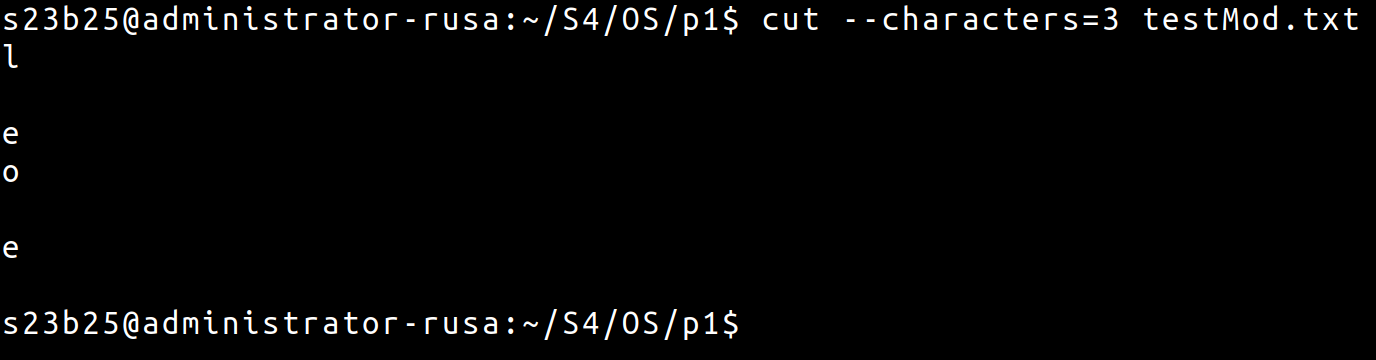
\includegraphics[width=\linewidth]{assets/cut-1.png}
\end{minipage}
} %output screenshot name
\end{figure}
